\documentclass[11pt, halfparskip]{scrartcl}

\usepackage[utf8]{inputenc}
\usepackage[T1]{fontenc}
\usepackage{ae}
\usepackage{amsmath}
\usepackage{graphicx}
\usepackage{booktabs}
\usepackage{listings}
\usepackage{subfig}
\usepackage{url}

\begin{document}

\lstset{numbers=none, tabsize=2, frame=tb, captionpos=t, basicstyle=\small}
\titlehead{

\includegraphics[scale=0.25]{graphics/iwb_logo}
}
\title{How to Implement a Server Plug-In}
\author{Felix Elliger\\ \url{fel@inubit.com}}
\date{}


\maketitle

\setcounter{tocdepth}{2} 
\tableofcontents

\cleardoublepage

\section{General Information and Classification of Plug-Ins}
\subsection{General Information}

Server plug-ins are located within the package
\verb!com.inubit.research.server.plugins!. 
There are two basic alternatives how users can access a plug-in's
functionality. 
If the plug-ins are connected to the model, they are accessible
for users via the "Plugins" - Button (see Fig.~\ref{screenshot}) of the web
editor's toolbar or via a toolbar icon. To connect a plug-in to certain model
types implement the \textit{ModelScope}-interface. To force a model plug-in to
be
rendered as a toolbar icon, override the \verb!showInToolbar()!-method within
your plug-in class.

If a plug-in is connected to specific object types, there is shown another
button within the object's context menu. To connect a plug-in to certain object
types implement the \textit{ObjectScope}-interface.

Currently, there have been no tests concerning the implementation of
both interfaces for one single plug-in class. From a server-side point of view
this should not raise any problem.

\begin{figure}[ht]
	\begin{center}
	\subfloat[][Toolbar]{
	  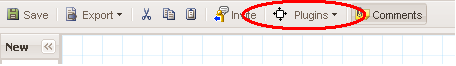
\includegraphics[width=0.6\textwidth]{graphics/screenshot}
	}\qquad
	\subfloat[][Context menu]{
	  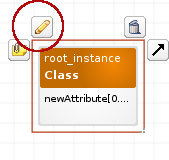
\includegraphics[width=0.25\textwidth]{graphics/screenshot2}
	}
	\end{center}
	\caption{Occurrences of plug-in icons}
	\label{screenshot}
\end{figure}

The implementer of a plug-in does not have to care about the URI that belongs
to his/her plug-in. A unique URI will be assigned at server start-up, or plug-in
registration. By now, there is no plug-in class that has configurable sub-URIs.
This will be implemented later when such a use-case exists.

\paragraph{How Do I Return the Plug-In's Response?}
Plug-in communication is entirely based on JSON as data interchange format.
Therefore, for returning the plug-in's response to the client you should always
use the method \verb!ResponseUtils.respondWithJSON!.

For more details on plug-in responses see Section \ref{response_section}.

\subsection{Classification of Plug-Ins}
Figure \ref{overview} shows the general classification of server plug-ins. All
of the depicted classes are abstract and 
have to be sub-classed for implementing a plug-in. As stated above, the
interfaces \textit{ModelScope} and \textit{ObjectScope} are used to connect the
plug-in to specific model classes or object classes respectively.

\begin{figure}[ht]
	\centering
	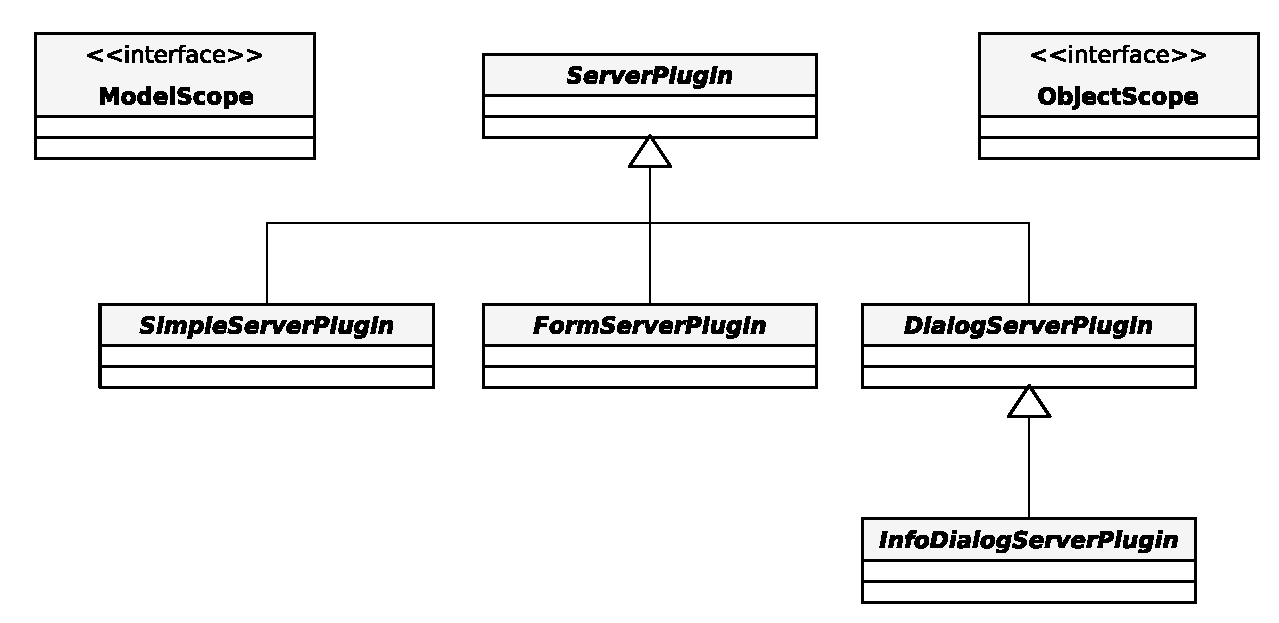
\includegraphics[width=0.8\textwidth]{graphics/pluginclasses}
	\caption{Classification of server plug-ins}
	\label{overview}
\end{figure}

Depending on its type the plug-in has a certain set of capabilities. These
capabilities and the required implementation effort is presented in the
following sections.

To capture the current model and its selection when calling the plug-in, there
exists the class \textit{ModelInformation}.
This class provides the following methods:
\begin{itemize}
	\item \verb!ProcessModel getProcessModel()! \\ Returns the current
process model the plug-in should use.
	\item \verb!Set<String> getSelectedNodes()! \\ Returns the IDs of
nodes that are selected within the current model.
	\item \verb!Set<String> getSelectedEdges()! \\ Returns the IDs of
edges that are selected within the current model.
\end{itemize}

As the implementer of a plug-in, you do not have to care about how this
information gets to your plug-in. The 
\textit{ModelInformation} object is created by the abstract classes and will be
passed to the respective methods.

\subsection{Item Offset Specification}
The \textit{ObjectScope}-interface provides a method \verb!getIconOffsetInfo()! returning an instance of the accordingly named class.
The information provided by an instance of this class determines the position of the plug-in's button within the object's context menu. Therefore, it specifies a general horizontal and vertical orientation along with a horizontal and vertical pixel offset.

The orientation is specified by the enum type \textit{Orientation}. It is recommended to use its values \verb!LEFT, RIGHT, CENTER! for horizontal orientation and \verb!TOP, BOTTOM, CENTER! for vertical orientation respectively.

As an example, the delete-button, that is rendered by default when a single object is selected would specify the following offset information:
\begin{itemize}
 \item horizontal orientation = \verb!TOP!
 \item horizontal offset = -11
 \item vertical orientation = \verb!RIGHT!
 \item vertical offset = -27
\end{itemize}
These values force the button to be rendered above the top right corner of the frame surrounding the selected object. The offset values have been carefully figured out by simple testing.



\cleardoublepage

\section{Simple Plug-Ins}
	\subsection{Overview}
		\begin{table}[ht]
			\centering
			\begin{tabular}{@{}lr@{}}
			\toprule
			\textbf{Required superclass} &
\textit{SimpleServerPlugin} \\
			\textbf{Configurable Sub-URLs} & \textit{no} \\
			\textbf{Requires JavaScript} & \textit{no} \\
			\textbf{Methods to implement} & \textit{void
performAction( ModelInformation mi , }\\
			& \textit{RequestFacade req , } \\
			& \textit{ResponseFacade resp , } \\
			& \textit{LoginableUser u )} \\
			\addlinespace
			& \textit{String getItemText()} \\
			\addlinespace
			& \textit{\textbf{(optional)} String
getItemIconPath()}\\
			\addlinespace
			\textbf{Graphical representation} & \textit{a single
menu item or context button} \\
			\textbf{Example(s)} & \textit{Layout} \\
			\bottomrule
			\end{tabular}
		\end{table}
	
	\subsection{Details}
		\subsubsection{Basic Information}
		Simple plug-ins are, as their name is already telling, the
simplest way of implementing a plug-in. Their graphical representation within
the editor's interface is limited to a single menu item within the
"Plugins"-menu, or directly within the editor's toolbar. The latter can be
achieved by overriding the \textit{showInToolbar()} method.
		
		If the user selects the menu item, a POST-request is generated
and sent to the plug-in's unique URL. The POST data consists of the current
model's ID along with the IDs of selected nodes and edges. In a first step this
JSON data is transformed into a \textit{ModelInformation} object which is then
passed to the \verb!performAction! method of your simple plug-in.
		
		\subsubsection{Methods}
			\paragraph{void performAction( ModelInformation mi,
RequestFacade req, ResponseFacade resp, LoginableUser u );}
			This method is responsible for processing the incoming
request and sending a resulting response to the requester.
			All required information has to be taken from the
\textit{ModelInformation} object. 
			
			See Section \ref{response_section} for information on
how responses must be structured.
			
			\paragraph{String getItemText();}
			Return the text for the menu item. If the
\textit{showInToolbar()}-method for this plug-in returns \verb!true! the item
text will be used as tool-tip text instead.

			\paragraph{String getItemIconPath();}
			Return the path to the icon of the menu item. This is
especially important if the plug-in is represented as a simple button within the
toolbar or as a context menu button.
			
			

\cleardoublepage

\section{Form Plug-Ins}
	\subsection{Overview}
		\begin{table}[ht]
			\centering
			\begin{tabular}{@{}lr@{}}
			\toprule
			\textbf{Required superclass} & \textit{FormServerPlugin}
\\
			\textbf{Configurable Sub-URLs} & \textit{no} \\
			\textbf{Requires JavaScript} & \textit{no} \\
			\textbf{Methods to implement} & \textit{void
performFormAction( RequestFacade req , } \\
			& \textit{ResponseFacade resp , } \\
			& \textit{MultiPartObject mpo , }\\
			& \textit{ModelInformation mi , }\\
			& \textit{LoginableUser u )} \\
			\addlinespace
			& \textit{JSONObject getFormConfig( ModelInformation mi , }
\\
			& \textit{RequestFacade req , } \\
			& \textit{LoginableUser u )} \\
			\addlinespace
			& \textit{\textbf{(optional)} String getItemText()} \\
			\addlinespace
			& \textit{\textbf{(optional)} String
getItemIconPath()}\\
			\addlinespace
			\textbf{Graphical representation} & \textit{a single
menu item or context button} \\
			\textbf{Example(s)} & \textit{Behavioral Interface
Generation,} \\
& \textit{Deploy to SolutionCenter} \\
			\bottomrule
			\end{tabular}
		\end{table}
	
	\subsection{Details}
		\subsubsection{Basic Information}
			As we can derive from the superclass name
\textit{FormServerPlugin}, this type of plug-in displays a form. As an advantage over simple plug-ins the entered form
data can be used while processing the users request. It is recommended to use this plug-in type, when the displayed form has to be generated dynamically. If the general shape of the form is indepent of a concrete model, or model state, please use \textit{DialogPlugin} as superclass (cf. Section \ref{dialog_plugins}).
			
			When the form is sent back to the server it is delivered
in a special format called multipart. For details on multipart see Section
\ref{multipart_format}. The implementer of the plug-in does not have to care
about parsing this format since that is done before the respective methods are
called.
		
		\subsubsection{Methods}
			\paragraph{void performAction(RequestFacade req,
ResponseFacade resp, MultiPartObject mpo, ModelInformation mi, LoginableUser u
);}
			After the form has been submitted, this method is responsible for processing the incoming
request and sending a resulting response to the requester.
			All available information is contained within the
\textit{ModelInformation} and the \textit{MultiPartObject} objects. The latter
contains the data the user entered into the form belonging to this plug-in. 
			
			See Section \ref{multipart_format} for information on
the multipart format.			
				
			See Section \ref{response_section} for information on
how responses must be structured.
			
			\paragraph{JSONObject getFormConfig(ModelInformation mi, RequestFacade req, LoginableUser lu)}
			Return a \textit{JSONObject} that configures the required form.
To facilitate this step there exist several classes within the package
\verb!com.inubit.research.! \verb!server.extjs!. Detailed information on these classes is
given in Section \ref{extjs}. Two buttons, "Submit" and "Cancel" are
automatically added to the form.
			
			\paragraph{String getItemText();}
			Return the text for the menu item. If the
\verb!showInToolbar()!-method for this plug-in returns \verb!true! the item text
will be used as tooltip text instead.

			\paragraph{String getItemIconPath();}
			Return the path to the icon of the menu item. This is
especially important if the plug-in is represented as a simple button within the
toolbar or as a context menu button.
	
		
		\subsubsection{ExtJS-Form Creation}
		\label{extjs}
		The creation of ExtJS form configurations is facilitated by the
\textit{ExtJSFormFactory} class. By calling 
		\verb!createEmptyForm()! you will receive an empty form to which
you can add all required items. As all objects returned by the factory extend the class \textit{JSONObject}, no further conversion is required.
		
		Supported ExtJS form elements are (further elements may be implemented):
		\begin{itemize}
			\item Container elements (can have multiple
sub-elements):
			\begin{itemize}
				\item FieldSet
				\item CheckboxGroup
			\end{itemize}
			\item Simple elements:
			\begin{itemize}
				\item Checkbox
				\item TextField
			\end{itemize}
		\end{itemize}
		
		For configuring these elements (and also the form itself) use
the respective \verb!setProperty! \verb!(key, value)! method. To view all
configurable attributes take a look at
\url{http://www.extjs.com/deploy/dev/docs/}.
		
		For accessing the entered data during request processing, you
have to specify the \textbf{name}-attribute for each simple element. This name
can then be used to get the corresponding value out of the created
\textit{MultiPartObject} instance.
			
		\subsubsection{Multipart Format}
		\label{multipart_format}
		When the user submits the form, the server receives the data in
multipart format. In a first step this format is transferred into a Java object
of type \textit{MultiPartObject}. Accessing this object will deliver the entered
data to the plug-in. 
		
		The following methods are considered to be helpful, where
\verb!mpo! is an instance of class \textit{MultiPartObject}, \verb!mi! is a
\textit{MultiPartItem}, and \verb!mp! is a \textit{SimpleMultipartParser}:
		\begin{itemize}
			\item \verb!mbo.getItems()!\\
			This returns all items contained in the multipart
object. That means, that all none empty (or unset) form elements are returned by
this call.
			\item \verb!mbo.getItemByName(String name)!\\
			Return one specific item that is identified by its
unique name. The name is taken from the \textbf{name}-attribute of the form
element. The form element is only found if the name exists and the element has a
none-\verb!null! value. For checkbox elements this means, that they are only
part of the submitted form if they were checked when submitting the form.
			\item \verb!mbi.getContent()!\\
			Get the textual content of a form element. This is equal
to the value the user entered into the specific field.
		
			\item
\verb!sp.parseItemContentAsByteArray(BufferedInputStream bis, String itemName)!\\
			Reads a specific item of the input stream as byte array.
This can be used, e.g., to parse an image
			
		\end{itemize}
		
\cleardoublepage

\section{Dialog Plugins}
\label{dialog_plugins}
	\subsection{Overview}
		\begin{table}[ht]
			\centering
			\begin{tabular}{@{}lr@{}}
			\toprule
			\textbf{Required superclass} & \textit{DialogServerPlugin}
\\
			\textbf{Configurable Sub-URLs} & \textit{no} \\
			\textbf{Requires JavaScript} & \textit{yes} \\
			\textbf{Methods to implement} & \textit{JSONObject
getData( ModelInformation mi , }\\
& \textit{RequestFacade req )} \\
			\addlinespace
			& \textit{JSONObject saveData( JSONArray data, }
\\
			& \textit{ModelInformation mi ) } \\
			\addlinespace
			& \textit{\textbf{(optional)} String getItemText()} \\
			\addlinespace
			& \textit{\textbf{(optional)} String
getItemIconPath()}\\
			\addlinespace
			\textbf{Graphical representation} & \textit{a single
menu item or context button} \\
			\textbf{Example(s)} & \textit{Domain Class Attribute Dialog} \\
			\bottomrule
			\end{tabular}
		\end{table}
	
	\subsection{Details}
		\subsubsection{Basic Information}
		This type of plug-in is similar to form plug-ins discussed within the last section. The main difference is that the basic structure of the dialog is specified within a JavaScript file (cf. Section \ref{dialog_script_info}). When the plug-in is loaded into the editor the required JavaScript file(s) is(are) loaded into the client and the dialog. If the respective menu item or button gets clicked, the dialog is instantiated and presented to the user within an Ext.Window.

		To ensure the described functionality, the implementer must take care of the following aspects:
		\begin{itemize}
		 \item The JavaScript dialog class must conform to the requirements specified in Section \ref{dialog_script_info}
		 \item The plug-in's constructor must set the field \verb!jsFiles!, to specify the JavaScript files that are specific for this plug-in.
		 \item The plug-in's constructor must set the field \verb!mainClassName!, specifying the name of the main JavaScript dialog class
		\end{itemize}

		In contrast to form plug-ins, the dynamic aspects of dialog plug-ins are reduced to loading and saving data using the respective methods.

		\subsubsection{Methods}
			\paragraph{JSONObject getData( ModelInformation mi, RequestFacade req );}
			 This method is responsible for collecting the data that should be loaded into the dialog. The concrete format of the data depends on the JavaScript implementations for this plug-in (cf. Section \ref{dialog_script_info}). The returned JSONObject must specify a field \verb!data! to which the data is associated.

			\paragraph{JSONObject saveData( JSONArray data,  ModelInformation mi );}
			This method is responsible for saving the data as it is returned from the client. The concrete format and number of the array entries depends on the JavaScript implementations for this plug-in (cf. Section \ref{dialog_script_info}). The returned JSONObject must be a valig plug-in response.
	
			See Section \ref{response_section} for information on how responses must be structured.
  
			\paragraph{String getItemText();}
			Return the text for the menu item. If the
\verb!showInToolbar()!-method for this plug-in returns \verb!true! the item text
will be used as tooltip text instead.

			\paragraph{String getItemIconPath();}
			Return the path to the icon of the menu item. This is
especially important if the plug-in is represented as a simple button within the
toolbar or as a context menu button.

		\subsubsection{JavaScript}
		\label{dialog_script_info}
		 The main JavaScript class, i.e. the class representing the dialog, must inherit from \verb!Ext.ux.Dialog!. This class, specifying 3 additional methods, is a sub-class of \verb!Ext.Panel! and, thereby, also provides all standard panel methods. Listing \ref{dialog_js} depicts the specification of \verb!Ext.ux.Dialog!.

		Please note, \verb!setData! must be coordinated with the implementation of the server-side method \verb!getData! since the therein specified data format must be processed by the JavaScript method. Accordingly, \verb!getJSONData! must be coordinated with the server-side method \verb!saveData! since the latter has to process the data created by the former.

		The method \verb!getTitle()! is a convenience function form determining the dialog's title.

		In case you are not familiar with ExtJS inheritance mechanism, take a look at \url{http://dev.sencha.com/deploy/dev/docs/?class=Ext}. The documentation of the method \verb!extend! presents the most important practical information.
		\clearpage
		\begin{lstlisting}[language=Java, caption=Ext.ux.Dialog, label=dialog_js]
Ext.namespace("Ext.ux");

Ext.ux.Dialog = Ext.extend( Ext.Panel, {
    constructor : function( config ) {
        Ext.ux.Dialog.superclass.constructor.call(this, config);
    },

    setData : function( data ) {
        //process the data returned by the server
    },

    getJSONData : function() {
	    / * 
	      * collect the data that should be sent to the server in 
	      * JSON format
	      * /
    },

    getTitle : function() {
        //return the title of this dialog
    }
});
		\end{lstlisting}

\cleardoublepage

\section{Info-Dialog Plug-Ins}
	  This class provides a minor extension of standard dialog plug-ins. The main difference is that the dialogs have only informational purpose but cannot be used to save modified data at the server. The specified dialogs are shown as tabs below the editor (see Figure \ref{info_dialog_screenshot}). Except for \verb!saveData()!, the implementer has to implement the same methods as for dialog plug-ins (cf. Section \ref{dialog_plugins}).

	\begin{figure}[ht]
	  \centering
	  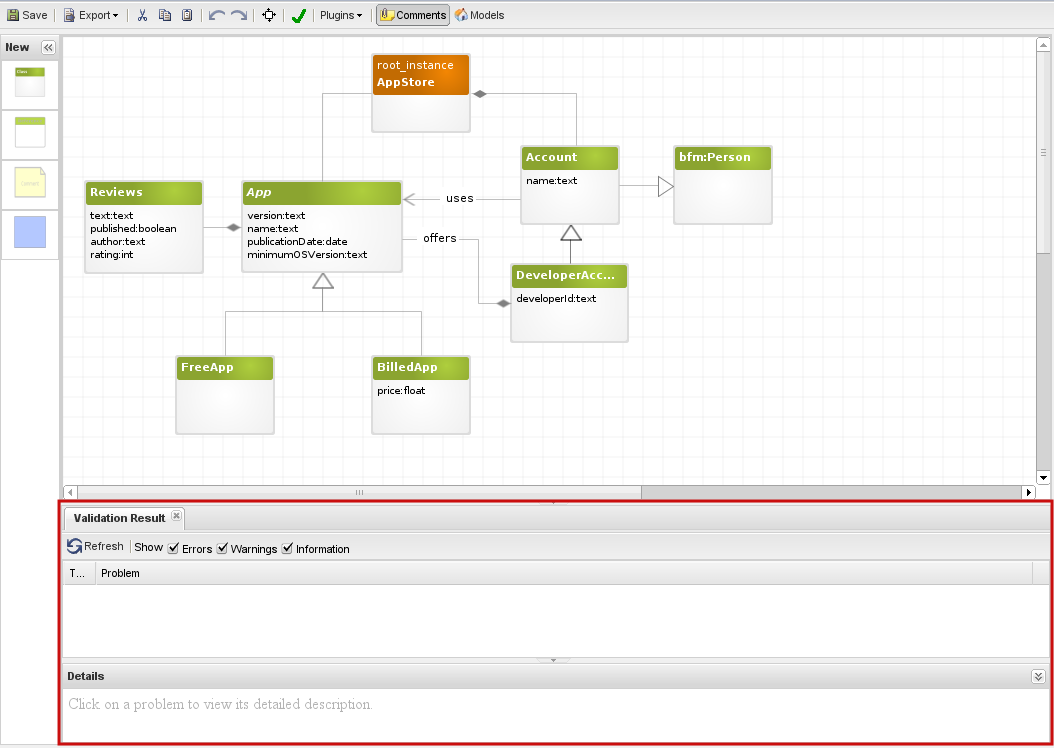
\includegraphics[width=0.8\textwidth]{graphics/info_dialog_screenshot}
	  \caption{Display area for info-dialog plug-ins}
	  \label{info_dialog_screenshot}
	\end{figure}

	\subsection{JavaScript}
	In contrast to standard dialog plug-ins, the main JavaScript class has to inherit from \verb!Ext.ux.InfoDialog!, which is itself an extension of \verb!Ext.ux.Dialog!. Listing \ref{infodialog_js} displays the source code of \verb!Ext.ux.InfoDialog!. As one can see, the dialog has access to the plug-in it is created for. Thereby, the dialog is able to refresh the displayed data by calling \verb!this.plugin.refreshData()!. This refresh mechanism can be used ,e.g., to implement a refresh button.
	\clearpage
	\begin{lstlisting}[language=Java, caption=Ext.ux.Dialog, label=infodialog_js]
Ext.namespace("Ext.ux");

Ext.ux.InfoDialog = Ext.extend( Ext.ux.Dialog, {
    constructor : function( config ) {
        Ext.ux.InfoDialog.superclass.constructor.call(this, config);
    },

    setPlugin : function( plugin ) {
        this.plugin = plugin;
    }
});
	\end{lstlisting}
	

\cleardoublepage

\section{Plug-In Responses}
\label{response_section}

The body of the HTTP response of a plug-in consists of a flag indicating the success of the operation, an action, and a data block that is required for processing the action. Responses are delivered in JSON format. The possible actions are listed in the enumeration \textit{PluginResponseType} which is contained in \verb!ServerPlugin.java!. The following sections describe each action in detail.

\subsection{OPEN - Action}
	\begin{table}[ht]
		\centering
		\begin{tabular}{@{}ll@{}}
			\toprule
			\textbf{Description} & Opens a new window or browser tab (depending on browser). \\
			& This can usually be used to open new models. \\
			\addlinespace
			\textbf{Required data} & The URI that should be opened. \\
			\bottomrule						
		\end{tabular}
	\end{table}
	
	\paragraph{Remark} To add new temporary models to the model manager and return the corresponding URL, the code of Listing \ref{newtmp} in Section \ref{code_examples} might help.
	
	\subsubsection{Response Format}
	\begin{lstlisting}
{
	success: true,
	action: 'OPEN',
	uri: '/your/valid/uri/starting/with/slash'
}
	\end{lstlisting}
	
\subsection{UPDATE - Action}
	\begin{table}[ht]
		\centering
		\begin{tabular}{@{}ll@{}}
			\toprule
			\textbf{Description} & Update the current model. This includes changes of node and edge\\
			&representations, their positions, as
			well as their creation, or removal.\\
			&Changes of element positions are animated. \\
			\addlinespace
			\textbf{Required data} & Model difference information. For details see the description in Section \ref{layout_data}\\
			\bottomrule						
		\end{tabular}
	\end{table}
	
	\subsubsection{Model Difference Data}
	\label{layout_data}
	Model difference data is used to communicate server side changes of a model to the editor. It states which nodes and edges have been changed, removed, or created and provides the necessary data. For details on the data format see class \textit{ModelDifferenceTracker}.
	
	Listing \ref{mdt} shows an example of how a \textit{ModelDifferenceTracker} can be used to collect the necessary information. 	
	\subsubsection{Response Format}
		\begin{lstlisting}
{
	success: true,
	action: 'UPDATE',
	data: <model difference data>
}
		\end{lstlisting}	
	
\subsection{INFO - Action}	
	\begin{table}[ht]
		\centering
		\begin{tabular}{@{}ll@{}}
			\toprule
			\textbf{Description} & Display an informative message to the user. \\
			& The generated dialog will show an INFO icon.\\
			\addlinespace
			\textbf{Required data} & The message that should be displayed.\\
			\bottomrule						
		\end{tabular}
	\end{table}
	
	\subsubsection{Response Format}
		\begin{lstlisting}
{
	success: true,
	action: 'INFO',
	infomsg: 'Your message to display'
}
		\end{lstlisting}
	
\subsection{ERROR - Action}
	\begin{table}[ht]
		\centering
		\begin{tabular}{@{}ll@{}}
			\toprule
			\textbf{Description} & Display an error message to the user. \\
			& The generated dialog will show an ERROR icon.\\
			\addlinespace
			\textbf{Required data} & The message that should be displayed.\\
			\bottomrule						
		\end{tabular}
	\end{table}
	
	\subsubsection{JSON Response Format}
		\begin{lstlisting}
{
	success: false
	action: 'ERROR',
	errormsg: 'Your message to display'
}
		\end{lstlisting}	
	
\cleardoublepage	

\section{Code Examples}
\label{code_examples}

\begin{lstlisting}[language=Java, label=newtmp, caption=Add a new temporary model to the model manager]
ProcessModel pm = <your code to get new model>;

String newUri = ModelManager.getInstance().addTemporaryModel(pm);
//newUri holds the complete URI relative to the server's root-URI
\end{lstlisting}

\begin{lstlisting}[language=Java, label=mdt, caption=Track model changes and create model difference JSON]
RequestFacade req;
ProcessModel pm = <your code to get new model>;

ModelDifferenceTracker mdt = new ModelDifferenceTracker( pm );
pm.addListener(mdt);

//apply your custom changes to the model

pm.removeListener(mdt);
JSONObject jo = mdt.toJSON(ModelRequestHandler
		                          .getAbsoluteAddressPrefix(req));
\end{lstlisting}

%\cleardoublepage
%\begin{lstlisting}[language=XML, label=layoutxml, caption=Example layout data]
%<data>
%	<bounds>
%		<property name='width' value='450'/>
%		<property name='height' value='700'/>
%	</bounds>
%	<objectupdates>
%		<nodes>
%			<node id='1237'>
%				<removed/>
%			</node>
%			<node id='373'>
%				<added/>
%			</node>
%			<node id='987'>
%				<property name='width' value='100'/>
%				<property name='height' value='70'/>
%				<property name='x' value='200'/>
%				<property name='y' value='260'/>
%			</node>
%			<node id='654'>
%				<imageuri value='/new/uri'/>
%				<property name='width' value='50'/>
%				<property name='height' value='50'/>
%				<property name='x' value='100'/>
%				<property name='y' value='160'/>
%			</node>
%		</nodes>
%		<edges>
%			<edge id='1'>
%				<removed/>
%			</edge>
%			<edge id='2'>
%				<added/>
%			</edge>
%			<edge id='3'>
%				<points>
%					<point x='1' y='1'/>
%					<point x='70' y='120'>
%				</points>
%			</edge>
%		</edges>
%	</objectupdates>
%</data>
%\end{lstlisting}	
\end{document}
